\documentclass[11pt]{article}
\usepackage{geometry}
\usepackage[utf8]{inputenc}
\usepackage[hidelinks]{hyperref}
\usepackage{natbib}
\usepackage{graphicx}
\usepackage{float}
\usepackage{amsmath}

\DeclareMathOperator*{\argmax}{argmax}
\DeclareMathOperator*{\logit}{logit}
\DeclareMathOperator*{\dnn}{DNN}


\begin{document}

\begin{titlepage}
    \begin{center}
        \vspace*{1cm}
        \begin{huge}
            Literature survey on \\ \textbf{Decoding with language models}
        \end{huge}
        
        \begin{large}
            \vspace{0.5cm}
            CS-E4070 End-to-end systems for speech recognition

            \vspace{1.5cm}
            Anssi Moisio, 474694
            
            \vspace{0.5cm}
            \today
        \end{large}
    \end{center}
    
\end{titlepage}

% Answer to questions:
% What is the topic you presented and how is it defined in the context of E2E ASR?
% What are the key concepts and how are they defined wrt E2E-ASR?
% What are some important results, conclusions, and future challenges in this topic?
% How can the work in this topic be categorized in terms of the concepts you defined?
% How do these different categories interact or compare in terms of system and its performance?

\section{Introduction}

An End-to-End (E2E) automatic speech recognition (ASR) system is trained on a parallel corpus of speech and transcription of the speech. Current E2E ASR systems, which are typically neural network models, require large numbers of data to train on. This poses a problem because transcribed speech data are arduous to produce and therefore expensive. The problem becomes crucial especially when training E2E ASR systems for low-resource languages that have few data to train the models on. In contrast to parallel corpora, text-only corpora are usually abundantly available even for low-resource languages. Therefore a proposed solution to the problem is to use text data to learn a language model, which can then be integrated into the E2E ASR system to provide information about the language at the decoding stage. This also enables domain transfer learning: an E2E ASR system can be trained on a source domain in which there are large parallel corpora available, and then transferred to a target domain by integrating a target domain language model to the system.
% For low-resource domains and languages, an E2E ASR system can be trained on another domain with more data available and then  
% (A semantic, or terminological, question is whether the resulting combined system is an E2E system anymore.)
% The external language model can be fused with the decoder in multiple ways. The next section describes some of the recently developed approaches.


\section{Background}
\subsection{Decoding with language models in traditional ASR}
Traditional ASR systems are influenced by the noisy channel model framework from information theory \citep{Jelinek1976}. In this framework, a \emph{source} (speaker) produces a piece of text. The task of a language model (LM) is to estimate the prior probability $P_{LM}(\boldsymbol{y})$ that a piece of text $\boldsymbol{y}$ is produced by the source. The piece of text then goes through a \emph{channel} that encodes it and transforms it into a sequence of of phonemes $\boldsymbol{x}$ which can be mapped to graphemes using a phoneme lexicon (also called dictionary).
The channel is modelled by an acoustic model that generates a probability distribution
\begin{equation}
    P(\boldsymbol{x}|\boldsymbol{y}) =
    \sum_{s \in S_{\boldsymbol{y}}}P(\boldsymbol{x}|\boldsymbol{s})
    P(\boldsymbol{s}|\boldsymbol{y}) =
    \sum_{s \in S_{\boldsymbol{y}}}\prod_t P(\boldsymbol{x}_t|\boldsymbol{s}(t)) 
\end{equation}
for acoustic features $\boldsymbol x = \boldsymbol x_1,...,\boldsymbol x_T$ given a piece of text $\boldsymbol y = y_1,..., y_U$, with possible time alignments $S_{\boldsymbol{y}}=\{...,s,...\}$ \citep{Mcdermott}. The prior alignments $P(\boldsymbol{s}|\boldsymbol{y})$ can be implemented using, for example, a Markov model.
A \emph{decoder} then determines the piece of text that has most probably caused the observed sequence, i.e. the output of the acoustic model mapped to graphemes. Using the Bayes' formula, this means maximising the posterior probability
\begin{equation}\label{bayes}
    P(\boldsymbol{y}|\boldsymbol{x}) = 
    \frac{P(\boldsymbol{x}|\boldsymbol{y})P_{LM}(\boldsymbol{y})} {P(\boldsymbol{x})}
\end{equation} 
where the probability of the acoustic features $P(\boldsymbol{x})$ can be ignored because it does not affect the maximum posterior, yielding the maximum posterior estimate
\begin{equation}\label{map}
    \hat{\boldsymbol{y}} = \argmax_{\boldsymbol{y}}
    P(\boldsymbol{x}|\boldsymbol{y})P_{LM}(\boldsymbol{y})
\end{equation} 
This approach works well for traditional ASR systems that use generative models for acoustic modelling, for example gaussian mixture models. However, if the generative model is replaced with a discriminative neural network model, it does not produce an acoustic likelihood $P(\boldsymbol{x}_t|\boldsymbol{s}(t))$ but a state level posterior probability $P(\boldsymbol{s}(t)|\boldsymbol{x}_t)$, which is a problem because the decoding (eq. \ref{map}) relies on the likelihoods. This mismatch can be bypassed by applying the Bayes' rule to produce pseudo-likelihoods:
\begin{equation}
    P(\boldsymbol{x}_t|\boldsymbol{s}(t)) =
    \frac{P(\boldsymbol{s}(t)|\boldsymbol{x}_t)P(\boldsymbol{x}_t)} {P(\boldsymbol{s}(t))} \propto	 
    \frac{P(\boldsymbol{s}(t)|\boldsymbol{x}_t)} {P(\boldsymbol{s}(t))}
\end{equation}
The state priors $P(\boldsymbol{s}(t))$ can be gathered from corpus frequencies \citep{Bourlard1994}. 



\subsection{Seq2Seq encoder-decoder for ASR}
E2E ASR systems map the input sequence $\boldsymbol x$ directly to text sequence $\boldsymbol y$ without decoupling the language model, the acoustic model and the phoneme to grapheme mapping. 
A common E2E speech recognition system architecture is that of a sequence-to-sequence (Seq2Seq) \citep{sutskever2014sequence} encoder-decoder. A Seq2Seq model maps an input sequence to an output sequence. In ASR, the input sequence is typically acoustic features extracted from a speech signal and the output sequence is typically characters, sub-word units, or words. The encoder creates a hidden representation $\boldsymbol h$ of the input sequence, and the decoder uses this representation to generate the probabilities of the output sequences
\begin{equation}
    P(\boldsymbol y|\boldsymbol x) = P(\boldsymbol y|\boldsymbol h) = 
    \prod_t P(y_t|\boldsymbol h, \boldsymbol{y}_{<t})
\end{equation}
Attention mechanisms, as introduced by \citet{bahdanau2014neural}, can be used between the encoder and the decoder to learn to locate and use the most relevant parts of the encoded hidden representation for the decoder to generate a certain part of the output sequence. An influential encoder-decoder model with attention for ASR was published by \citet{chan2016listen}, called Listen, Attend and spell (LAS). In this model, the attention mechanism calculates a context vector $\boldsymbol{c}_t = AttentionContext(\boldsymbol{d}_{t},\boldsymbol{h})$ for each time step. The current decoder state $\boldsymbol{d}_{t}$ is determined by the previous context vector $\boldsymbol{c}_{t-1}$, previous decoder state $\boldsymbol{d}_{t-1}$, and the previously emitted output $\hat{\boldsymbol{y}}_{t-1}$ 
\begin{equation}
    \boldsymbol{d}_{t} =
    RNN(\hat{\boldsymbol{y}}_{t-1}, \boldsymbol{d}_{t-1}, \boldsymbol{c}_{t-1})
\end{equation}
where $RNN$ is a 2 layer LSTM (Long Short-Term Memory) network.
The decoder  outputs the posterior distribution at a time step $t$ after a final layer
\begin{equation}
    P(y_t|\boldsymbol h, \boldsymbol{y}_{<t}) =
    softmax(\boldsymbol{W}_s[\boldsymbol{d}_{t}, \boldsymbol{c}_t] + \boldsymbol{b}_s)
\end{equation}
where $\boldsymbol{W}_s$ and $\boldsymbol{b}_s$ are learnable parameters.



\section{LM integration approaches}
\subsection{Shallow fusion and density ratio approach}
In the LM integration approach that \citep{gulcehre2015using} termed \emph{shallow fusion} in contrast to \emph{deep fusion}, the LM and ASR model output scores are combined to compute the output sequence similarly to the traditional ASR systems (eq. \ref{map}):
\begin{equation}
    \hat{\boldsymbol{y}} = \argmax_{\boldsymbol{y}} \log P(\boldsymbol{y}|\boldsymbol{x}) + \lambda \log P_{LM}(\boldsymbol{y}) \label{shallowfusion}
\end{equation}
% where $P(\boldsymbol{y}|\boldsymbol{x})$ is the probability that the Seq2Seq model assigns to the output sequence $\boldsymbol{y}$ given the input sequence $\boldsymbol{x}$.
where $\lambda$ is a tunable language model weight, and the logarithmic probabilities are used to avoid numeric underflow.

\begin{figure}[htb]
    \begin{center}
        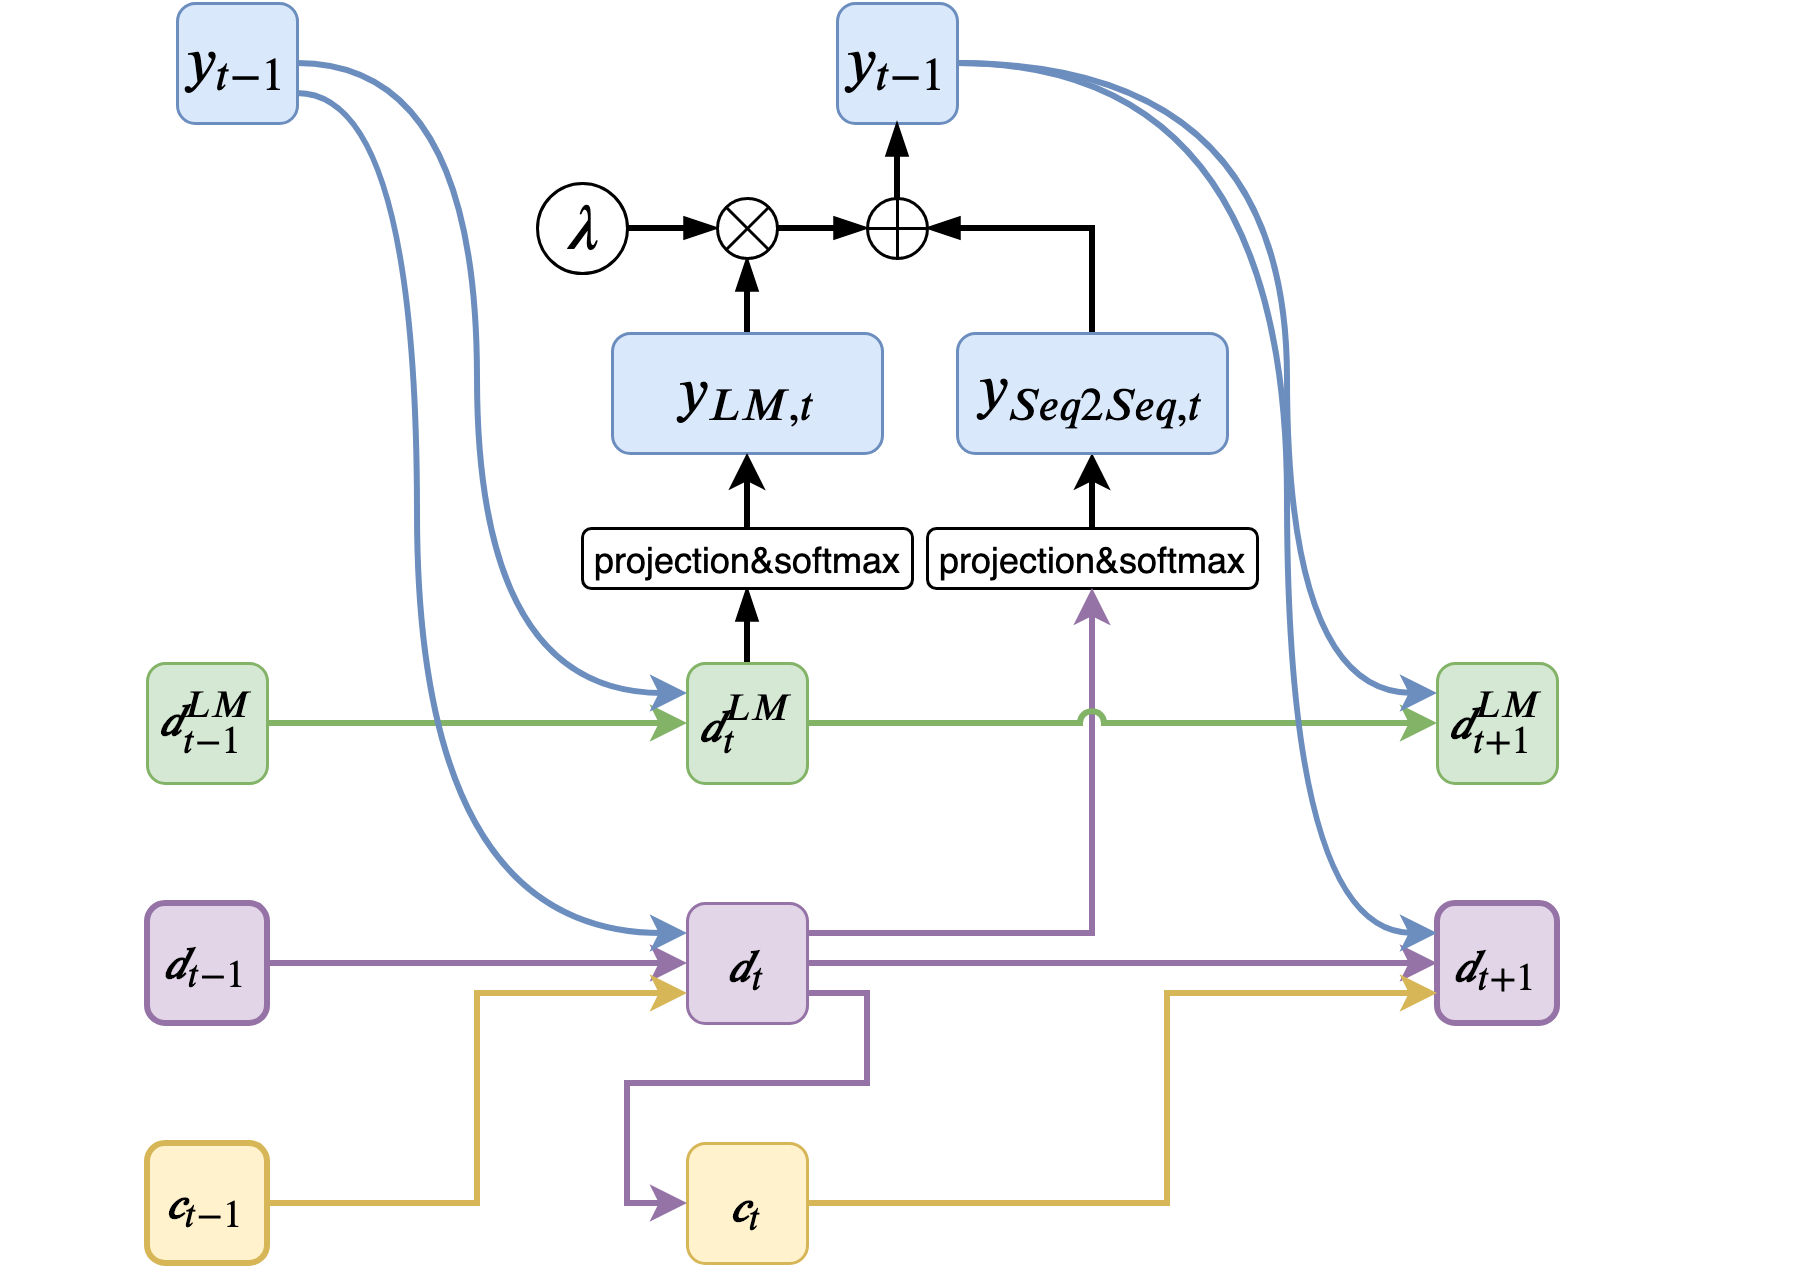
\includegraphics[height=8cm]{shallow.png}
    \end{center}
    \caption{Shallow fusion decoding step. The LM and Seq2Seq model outputs are combined.}
    \label{deepfusion}
\end{figure}

In practice,  $\log P(\boldsymbol{y}|\boldsymbol{x})$ is typically approximately maximized using a left-to-right beam search algorithm that produces a list of $K$ candidates for $\boldsymbol{y}$.
The combined score $\log P(\boldsymbol{y}|\boldsymbol{x}) + \lambda \log P_{LM}(\boldsymbol{y})$ is calculated only for $K$ candidate hypotheses $\{\hat{\boldsymbol{y}}^{(i)}\}_{i=1,...,K}$ with the top scores given by the decoder from the complete hypothesis space.
% Alternatively, the combined score of eq. \ref{shallowfusion} can be maximised using beam search.
% Shallow fusion is similar to the traditional ASR method of combining the acoustic model scores with the language model scores.



The shallow fusion approach can be extended to a density ratio approach if we have language models for both the source and target domain \citep{Mcdermott}. In this approach, the Seq2Seq probability is combined with the density ratio of the target and source domain probability distributions, instead of the single LM probability distribution as in shallow fusion. The division by the source domain LM output is a subtraction in the log domain:
\begin{equation}
    \hat{\boldsymbol{y}} = \argmax_{\boldsymbol{y}} \log P(\boldsymbol{y}|\boldsymbol{x}) + \lambda_{target} \log P_{LM,target}(\boldsymbol{y}) - \lambda_{source} \log P_{LM,source}(\boldsymbol{y}) \label{shallowfusion}
\end{equation}
Here the Seq2Seq model is trained on the source domain parallel (audio, transcript) corpus and the source domain LM is trained on the same transcripts.




\subsection{Deep fusion}

In shallow fusion, the LM is weighted uniformly with the scalar $\lambda$ across all hypotheses. Intuitively, however, the language model is more useful when decoding some sequences than others, and should therefore be weighted depending on the sequence. This requires the language model to be integrated to the decoder at an earlier stage of the encoder-decoder model. \citet{gulcehre2015using} introduced a method called deep fusion, in which the hidden states of the language model are concatenated with the hidden states of the decoder (see Figure \ref{deepfusion}). Like shallow fusion, deep fusion assumes that the ASR and LM models are pretrained, but deep fusion incorporates a learned controller mechanism
\begin{align}
    g_t = \sigma(\boldsymbol{v}_g^T\boldsymbol{d}_t^{LM}+b_g)
\end{align}
to weight the language model differently depending on the LM hidden state $\boldsymbol{d}_t^{LM}$. $\boldsymbol{v}_g^T$ and $b_g$ are the weight and bias that are learned in the fine tuning and $\sigma$ is the sigmoid squashing function. During the fine tuning of the integrated system, the context $\boldsymbol{c}_t$, decoder hidden state $\boldsymbol{d}_t$, and the weighted hidden state of the language model $g_t\boldsymbol{d}_t^{LM}$ are all concatenated to create the hidden state of the deep fusion layer $\boldsymbol{d}_t^{DF}$. The $\boldsymbol{d}_t^{DF}$ is parametrised with $\boldsymbol{W}_{DF}$ and $\boldsymbol{b}_{DF}$ and fed through a softmax layer to generate the conditional distribution output:
\begin{align}
    \boldsymbol{d}_t^{DF} &= [\boldsymbol{c}_t; \ \boldsymbol{d}_t; \ g_t\boldsymbol{d}_t^{LM}] \\
    P(y_t|\boldsymbol{h}, \boldsymbol{y}_{<t}) &= softmax(\boldsymbol{W}_{DF} \boldsymbol{d}_t^{LM} + \boldsymbol{b}_{DF})
\end{align}
The weight matrix $\boldsymbol{W}_{DF}$ and the bias $\boldsymbol{b}_{DF}$ are also learned in fine tuning. The integrated system is trained while keeping the parameters of the pre-trained ASR and LM models fixed so that the decoder learns to use the hidden states of the LM during the inference of the next word.

\begin{figure}[htb]
    \begin{center}
        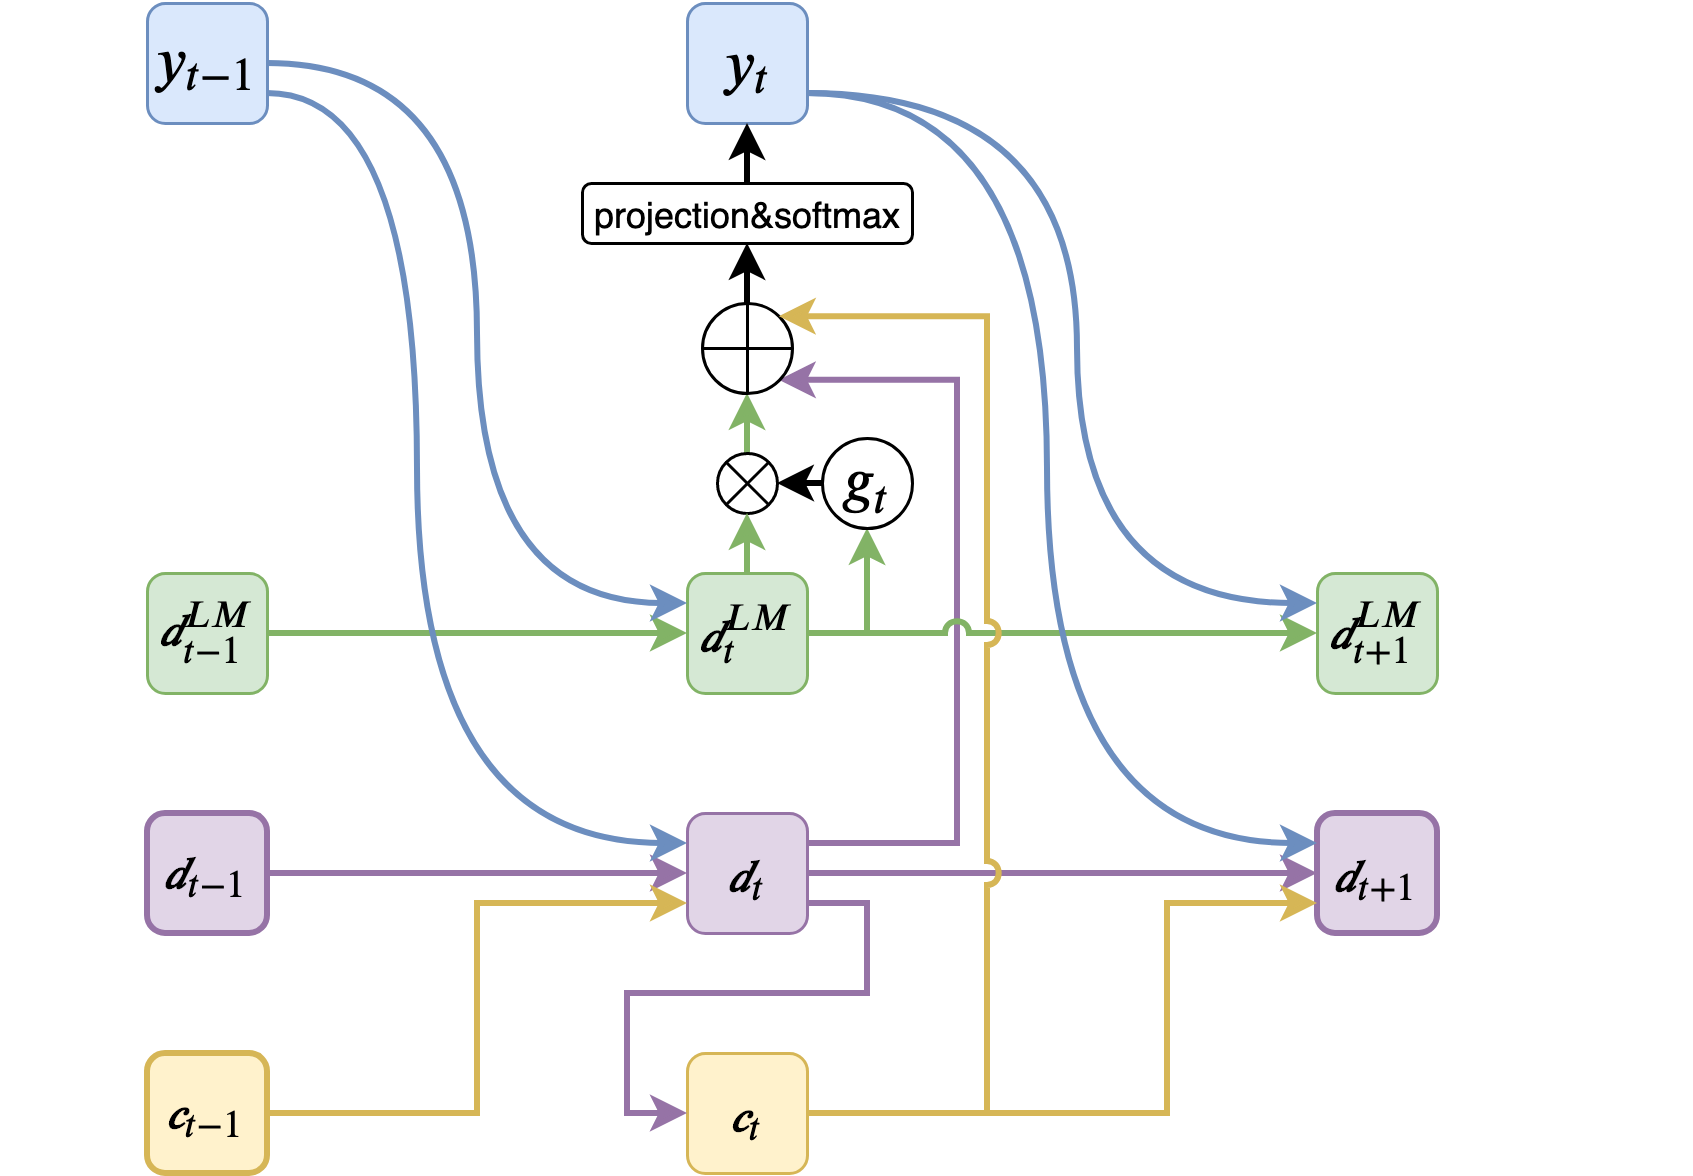
\includegraphics[height=7cm]{deepfusion.png}
    \end{center}
    \caption{Deep fusion decoding step. Gating function $g_t$ weights the language model state $\boldsymbol{d}_t^{LM}$, which is concatenated with the context vector $\boldsymbol c_t$ and the decoder state $\boldsymbol{d}_t$.}
    \label{deepfusion}
\end{figure}

Deep fusion was originally developed for neural machine translation (NMT), so it is motivated by properties of the translation problem. \citet{gulcehre2015using} give an example when the language model can be more useful in an NMT system: when translating from a language with no articles (a, an, the), such as Chinese, to English, the LM is probably useful in generating the articles because there are no Chinese words that correspond to articles. In contrast, when translating a noun, the LM is probably not as informative. When deep fusion is used in the ASR task, the LM is informative, for instance, when transcribing homophones, such as "two" and "too", and not so informative when transcribing phonetically unambiguous words.



\subsection{Cold fusion}

In both shallow and deep fusion, the ASR model is initially trained separately from the language model which means that it learns an implicit language model to transcribe the speech. When the external LM is integrated to the system, the implicit LM of the ASR model becomes redundant.
% , assuming the external LM is better.
This can be viewed as waste of the decoder capacity. Furthermore, the implicitly learned LM can be overfitted, or at least somewhat biased, to the relatively small corpus of transcribed speech. \citet{sriram2017cold} developed a method called Cold Fusion, in which the Seq2Seq encoder-decoder is trained to use an external language model from the beginning of the training instead of only at a fine-tuning stage as in deep fusion. This way the Seq2Seq learns to model only the acoustics and rely on the external LM for language information.

\begin{figure}[htb]
    \begin{center}
        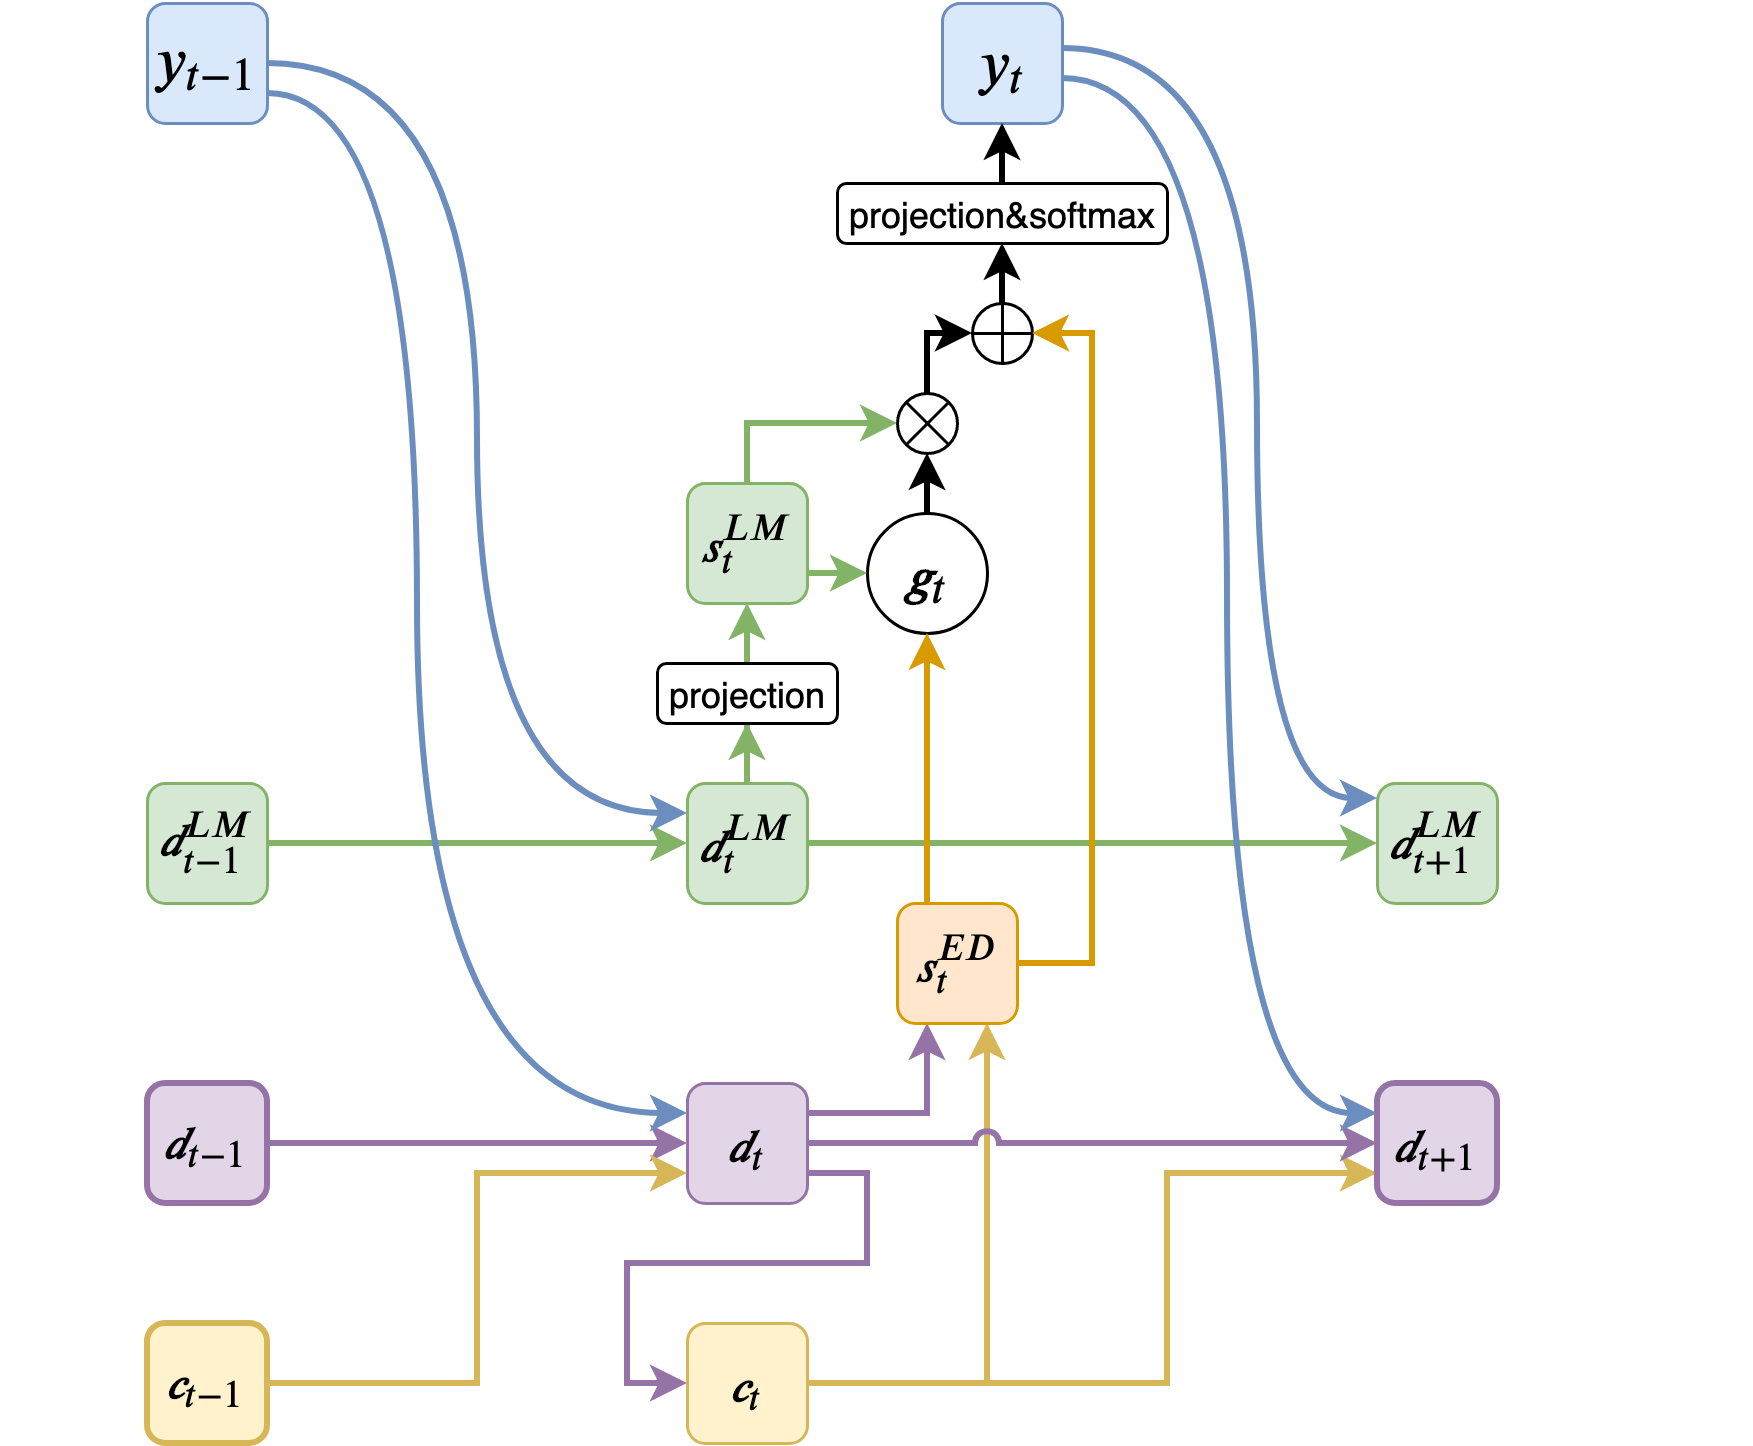
\includegraphics[height=9cm]{coldfusion.png}
    \end{center}
    \caption{Cold fusion decoding step. The gating function $\boldsymbol g_t$ is a vector, and it depends on both the enc-dec state $\boldsymbol{s}_t^{ED}$ and the projected language model logit output $\boldsymbol{s}_t^{LM}$.}
    \label{plot}
\end{figure}

In addition to the early training integration method, there are a number of other differences between deep and cold fusion.
In cold fusion, the language model hidden state $\boldsymbol{d}_t^{LM}$ as used in deep fusion is replaced by the language model logit probability fed through a DNN to create a projection to an embedding space that is uniform across different LMs.
The LM hidden state distribution and dynamics can vary considerable across different language models and data, making it impossible to change the LM. This projection enables switching to use a different LM:
\begin{align}
    \boldsymbol{s}_t^{LM} &= DNN(\logit P_{LM}(\boldsymbol{y}))
\end{align}

% \begin{align}
% \boldsymbol{s}_t^{ED} &= \boldsymbol{W}_{ED}[\boldsymbol{d}_t ; \ \boldsymbol{c}_t] + \boldsymbol{b}_{ED} \\
% \end{align}

Furthermore, cold fusion uses the fine-grained gating \citep{yang2016words} mechanism (equation \ref{finegrained}), making $\boldsymbol{g}_t$ a vector instead of a scalar as in deep fusion:
\begin{align}
    \boldsymbol{g}_t &= \sigma(\boldsymbol{W}_g[\boldsymbol{s}_t^{ED} ; \ \boldsymbol{s}_t^{LM}]+\boldsymbol{b}_g) \\
    \boldsymbol{s}_t^{CF} &= [\boldsymbol{s}_t^{ED}; \ \boldsymbol{g}_t \circ \boldsymbol{s}_t^{LM}] \label{finegrained}
\end{align}
where $\circ$ represents the element-wise (also called Hadamard) product of the vectors. The fact that the gating function $\boldsymbol{g}_t$ depends both on the LM hidden state $\boldsymbol{s}_t^{LM}$ and the decoder hidden state $\boldsymbol{s}_t^{ED}$ makes it possible to weight the LM more in situations where the acoustic signal is noisy, for instance, even though the LM would not have a large weight based only on the LM state as in deep fusion. Furthermore, the fine-grained gating allows for more flexibility in choosing which aspects of the LM state $\boldsymbol{s}_t^{LM}$ are emphasised at each time step, since the gating $\boldsymbol{g}_t$ weights each node of the LM state $\boldsymbol{s}_t^{LM}$ individually.

The cold fusion state $\boldsymbol{s}_t^{CF}$ goes through the final layers of the decoder to produce the output probability distribution:
\begin{align}
    \boldsymbol{r}_t^{CF} &= \dnn(\boldsymbol{s}_t^{CF}) \\
    P(y_t|\boldsymbol{h}, \boldsymbol{y}_{<t}) &= softmax(\boldsymbol{W}_{CF} \boldsymbol{r}_t^{CF} + \boldsymbol{b}_{CF})
\end{align}





\subsection{Decoder trained on multitask objective}

When the decoder input vector is set as a zero context vector, the Seq2Seq decoder objective function reduces to the LM objective function, i.e. the probability distribution of the next output symbol depends only on the previous state of the decoder and not on the encoder output. This allows for training the decoder on a multi-task objective, in which it learns the language modelling task and the usual Seq2Seq decoding task. The objective at each iteration is sampled from the set of two objectives according to some prior weights. When the decoder is trained on the language modelling task, the encoder and attention parameters are not affected.



\subsection{LM as a decoder layer}
\citet{toshniwal2018comparison} proposed also using an external language model as a lower decoder layer. The LM layer is placed to the decoder of a pretrained LAS models and the whole model is then fine-tuned on the LAS objective for a few epochs. Similar methods have been proposed by \citet{Ramachandran2017} and \citet{Rao2018} who used a pretrained LM as a lower decoder layer in a machine translation model and as the initialisation weights for an RNN transducer for speech recognition, respectively.





\section{Experiments}

This section reviews the experiments presented in by \citet{sriram2017cold} and \citet{toshniwal2018comparison}. The experiments were designed to determine which LM integration method achieves the best results in terms of word error rate (WER) or character error rate (CER). However, the experiment setups were not uniform, so no clear comparisons can be made.

\subsection{\citet{sriram2017cold}}
\subsubsection{Experiment setup}
\citet{sriram2017cold} performed single-domain and domain transfer experiments. For single domain, they used the LibriSpeech data set of audiobooks (960 hours) and non-overlapping text corpus of 800M tokens (900k unique words) from 14500 books \citep{panayotov2015librispeech}. They also added noise to this data to test the noise robustness of the models. For the domain transfer experiments, they collected a corpus of search queries and a corpus of movie transcripts respectively for source and target domains. Their source data set contained 411k utterances (650 hours), and target dataset 345k utterances (676 hours).

They had three main models that they compared: a baseline attention based encoder-decoder with no external language model, a deep fusion model, and a cold fusion model.

The LM for the single domain experiments trained on the Librispeech data consisted of one layer of 1536-dimensional GRUs. The LM for the  domain transfer experiments trained on the search query and movie transcript data consisted of three layers of 1024-dimensional GRUs. They used 40 mel scale filterbank features as input and characters as output.

\subsubsection{Results}
In the single domain experiments, using clean speech data the baseline attention ASR system got better results than deep fusion, whereas when using noisy data deep fusion got better results. This is in line with the idea that deep fusion enables the decoder to rely more on the language model when the speech is noisy, making this approach more robust to noise. However, cold fusion performed better than shallow or deep fusion on both clean and noisy speech. This can be because the decoder capacity is used more effectively, utilising the external language model better because of the more fine-grained integration.

Because the deep fusion approach uses the language model hidden state $\boldsymbol{d}_t$ instead of the projected output probabilities as in cold fusion, switching the language model is not possible. This makes domain transfer harder since the language model cannot be simply changed from one trained on the source domain to another trained on the target domain. For this reason they used a single LM for the fusion models. The cold fusion approach got better results than shallow or deep fusion in both source and target domain. The cold fusion approach is more complicated than the other two, including a projection of the LM model state and also a DNN before the final softmax layer after the concatenation of the language model output projection and Seq2Seq model state. This means that cold fusion requires more parameters than the other two approaches, which naturally affects the performance.

\citet{sriram2017cold} performed also some ablation studies on the deep and cold fusion approaches. They noted that the projection of the language model output helped especially in the domain transfer tests.

The main reasoning behind training the Seq2Seq model to utilise the LM from the beginning was that the decoder capacity would be used more efficiently to learn the Seq2Seq task rather than learning an implicit language model. They experimented reducing the size of the decoder, and noted that the cold fusion model was able to perform well with a smaller decoder size compared to deep fusion.




\subsection{\citet{toshniwal2018comparison}}
\subsubsection{Switchboard data}
\citet{toshniwal2018comparison} used two different speech data types in their experiments. First, they used the Switchboard (SWB) corpus of 300h / 192k utterances of conversational telephone speech and did the evaluation on SWB and CallHome (CH) corpora. They trained the language models on text from the SWB and Fischer corpora with 2M utterances. With these data, they used a model with 4-layer BLSTM 256-dimensional encoder, one-layer LSTM decoder, and one-layer 512-dimensional LSTM language model. They used 40 mel scale filterbank features with deltas and a 1000 BPE wordpiece vocabulary.

\subsubsection{Google voice search and dictation data}
Second, they used the Google voice search and dictation dataset of 22M utterances. They trained a larger model on this dataset: 5-layer unidirectional LSTM network (1400 dimensions) as encoder, 2-layer unidirectional LSTM (1024 dimensions) as decoder, and 2-layers of 2048-dimensional LSTM cells
as the language model. They extracted 80 mel scale filterbank features as the input and had a 16384 BPE wordpiece vocabulary as the output.

\subsubsection{Results}

In the experiments of \citet{toshniwal2018comparison}, shallow fusion performed the best on the SWB data and on the voice search data. On the dictation data, shallow fusion and cold fusion got similar results. The reason why cold fusion did not achieve the best results on these experiments as it did on the experiments of \citet{sriram2017cold}, could be that the latter used more parameters in the cold fusion layer than in other fusion approaches.
% Another reason might be that the 

\citet{toshniwal2018comparison} evaluated also the methods of using a pretrained LM as a decoder layer or training the decoder on  the multi-task objective (LM and Seq2Seq). They got some improvement on the LAS baseline by using each of these methods. The LM as decoder layer approach got better results than the multitask approach. Interestingly, LM as a decoder layer got similar results as the deep fusion and cold fusion approaches in these experiments.

When using a larger LM for rescoring the top-8 hypotheses of the beam search algorithm, the cold fusion approach achieved the best results. It is hard to know exactly why this fusion approach produces better top-8 lists than the other approaches.


\section{Conclusion}

% What are some important results, conclusions, and future challenges in this topic?
% How can the work in this topic be categorized in terms of the concepts you defined?
% How do these different categories interact or compare in terms of system and its performance?

% The two different articles in the last section got differing results from their experiments. In the experiments of \citet{sriram2017cold}, the cold fusion method achieved consistently the best results.

A few different approaches to integrating an external LM to an E2E ASR system has been recently proposed. The simplest method, shallow fusion, is to combine the output probabilities of the two models by a weighted linear combination in log domain. More complicated approaches, deep and cold fusion, fuse the hidden states of the two models together (or the hidden state of the Seq2Seq model and the projected output of the LM as in cold fusion) to utilise the LM and the Seq2Seq model more effectively, weighting the LM more when it is more useful, weighting different LM nodes differently (fine-grained gating), or utilising the pretrained LM in the Seq2Seq model training.

The more complicated fusing approaches (deep and cold) require additional layers and more stages in the training of the combined models, which makes them more expensive than the shallow fusion approach. However, the more complicated methods do not necessarily get better results than shallow fusion \citep{toshniwal2018comparison}. This would mean that the shallow fusion is the most cost-effective approach, being the simplest.

Although it is not clear which one of LM integration methods is the best, in general integrating an external language model by any of these methods brings improved results over the baseline LAS model without an external LM, at least with noisy data or in domain transfer tasks  \citep{toshniwal2018comparison, sriram2017cold, Mcdermott}.

The different fusion methods might be useful in different scenarios. The cold fusion approach is in theory able to utilise the external language model the most since it is fused in the system in the earliest stage, and it is fused with a more fine-grained gating mechanism. This might make the cold fusion most attractive method for domain transfer when there is a parallel corpus in a source domain and a sufficiently large text corpus in the target domain.




\bibliographystyle{apalike}
\bibliography{references}

\end{document}  